\documentclass{article}
\usepackage[left=0.85in, right=0.85in, top=0.5in, bottom=0.95in]{geometry}
\usepackage[T1]{fontenc}
\usepackage[utf8]{inputenc}
\usepackage[italian]{babel}
\usepackage{pdfpages}
\usepackage{graphicx}
\usepackage{wrapfig2}
\usepackage{amsmath}
\usepackage{amsthm}
\usepackage{amssymb}
\usepackage{cases}
\usepackage{gensymb} %simboli come ° = \degree  etc etc
\usepackage{subcaption}
\usepackage{hyperref}
\hypersetup{
	colorlinks=true,
	linkcolor=blue,    
	urlcolor=blue,
	%pdfpagemode=FullScreen,
}
\urlstyle{same}
\usepackage{changepage}
\usepackage{lastpage, epstopdf}
\usepackage{fancyhdr}
\usepackage{tcolorbox}
%\usepackage{background}
\usepackage{tikz}
\usetikzlibrary{patterns}


%=======HEADER & FOOTER=======%
\def\lesson{Lezione N. 12}
\def\outcome{\textbf{Learning Outcomes:} Outcomes go here. }

\pagestyle{fancy}
\fancyhf{}
\renewcommand{\headrulewidth}{0pt}
\renewcommand{\footrulewidth}{1.4pt}
\lfoot{A.M. $\diamond$ \the\year}
\cfoot{Page \thepage}
\rfoot{\lesson}

%=======CORNELL STYLE FORMAT=======%
%\SetBgScale{1}
%\SetBgAngle{0}
%\SetBgColor{black}
%\SetBgContents{\rule{1pt}{0.85\paperheight}}
%\SetBgHshift{-1.6in}
%\SetBgVshift{-0.1in}

%=======CUSTOM BOXES=======%

\parindent 0ex

%=======BODY=======%
\begin{document}
	\setcounterpageref{secnumdepth}{0}
	\section*{Parte 8} %Date: \hrulefill}
%	\begin{tcolorbox}{\outcome}\end{tcolorbox}

\begin{adjustwidth}{2in}{} 
	
\textbf{{\Large Concentrazione delle tensioni}} \mbox{} \newline
		Fin'ora si sono sempre considerate condizioni ideali: tutti i componenti erano regolari con geometrie date da estrusioni di sezione per cui le variazioni di forma erano ridotte. \newline 
		
		Nella realtà gli oggetti sono più complicati e gli stati tensionali più complessi, questi e sono facilmente influenzati da  elementi chiamati genericamente intagli, ovvero brusche variazioni di forma, discontinuità del materiale o effetti localizzati. 
		
		Le discontinuità possono dipendere  dallo stato del materiale, dal processo di realizzazione o dal trattamento termico, si possono identificare macroscopicamente, come la soffiatura data da una materozza mal dimensionata, o microscopicamente come la presenza di precipitati o di variazioni morfologiche di bordo grano. 
		Sia macrodiscontinuità che microdiscontinuità perturbano la condizione nominale dello stato di tensione. 
		
		Per materiali disomogenei come le ghise grige per valutare gli effetti di queste discontinuità si attribuisce una proprietà omogenea molto bassa, per materiali più omogenei l'effetto della variazione di tensione per concentrazione di tensione si valuta attraverso gli \textbf{intagli}.  \newline 
		
		Un intaglio è un difetto superficiale come può essere una scalfitura accidentale o una variazione di forma che rende molto più che complesso risolvere lo stato tensionale nell'intorno di quel punto attraverso la teoria elastica. \newline
		
		L'approccio classico allo studio delle concentrazioni di tensione è attraverso un fattore amplificativo $K_t$, coefficiente di concentrazione tensionale teorico/geometrico:
		\[K_t - \dfrac{\text{Tensione massima vera}}{\text{tensione nominale}}\]
		Dove la Tensione nominale $sigma_n$ altro non è che la
		sollecitazione presente se non sussistono concentrazioni locali di tensione (calcolata in assenza di
		concentrazione o talvolta in assenza di intaglio). 
		
		Questo parametro è funzione esclusivamente della geometria e varia a seconda della tipologia di sollecitazione. In nessun modo il $K_t$ dipende dall'entità del carico, è un termine adimensionalizzato rispetto alla tensione nominale. non è funzione del materiale, ma funzione della tipologia del materiale si deciderà se utilizzarlo o meno. \newline 
		
		Il $K_t$ sostanzialmente si applica secondo l'assunto per il quale il materiale raggiunge la criticità laddove la massima tensione raggiunga il livello critico, questo però è il criterio di Rankine e si applica ai materiali fragili! Le applicazioni meccaniche-industriali trattano anche materiali duttili! \newline 
		
		Il coefficiente $K_t$ va ad amplificare esclusivamente la massima delle tensioni presenti in quel punto, la tensione nominale. \newline 
		
		Tale tensione nominale può essere netta \textit{Net Stress} NS o lorda \textit{Gross Stress} GS. \newline 
		
		La NS è la tensione che si avrebbe nella sezione resistente contenente l'intaglio qualora fossero negati gli effetti di concentrazione di tensione. 
		
		Nell'esempio sottostante su di una piastra è praticato un foro per cui in prossimità di esso ci sarà una concentrazione di tensioni, il valore della massima tensione si ha proprio in corrispondenza del foro e sarà dato da $K_t\cdot\sigma_n$. 
		
		L'approccio con NS, tipico della letteratura italiana, dice che la tensione nominale è la tensione che si avrebbe su questa sezione data da "larghezza meno foro" immaginando l'assenza di concentrazioni, quindi con un carico uniforme. 
		
		Nella letteratura anglosassone vince invece l'approccio GS dove la tensione nominale è null'altro che la tensione che si avrebbe sulla sezione in assenza dell'intaglio. 
		
		\begin{figure}[H]
			\centering
			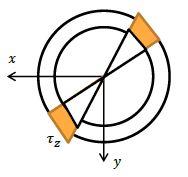
\includegraphics[width=0.5\linewidth]{immagini/screenshot001}
			\label{fig:screenshot001}
		\end{figure}
		
		
		In altre parole, la \textit{Net Stress} nega le concentrazioni di tensioni e considera una sezione ridotta, mentre la \textit{Gross Stress} considera la tensione nominale senza la presenza dell'intaglio.\newline 
		
		Cambierà perciò il valore rispetto al quale si normalizzerà il $K_t$, per questo sarà riportato in didascalia alle tabelle la scelta di tensione nominale utilizzata. \newline 
		
		Si immagini ora di confrontare le linee di forza sulla piastrina con le linee di flusso idrodinamiche (analogia idrodinamica tanto più valida tanto più si parla di sforzi di taglio), come queste si addensano vicino al foro, per mantenere la continuità, la velocità del flusso aumenta, cosi come la tensione: sarà proprio vicino al foro che si avrà il massimo valore di tensione. \newline 
		
		Si consideri un cilindro con intaglio posto a trazione. La tensione principale per un cilindro caricato assialmente dovrebbe essere una, ebbene, qui se ne contano tre: una $\sigma_a$ assiale, una $\sigma_r$ radiale/normale (a causa del sistema di riferimento cilindrico) e $\sigma_t$ tangenziale/circonferenziale. 
		
		\begin{figure}[H]
			\centering
			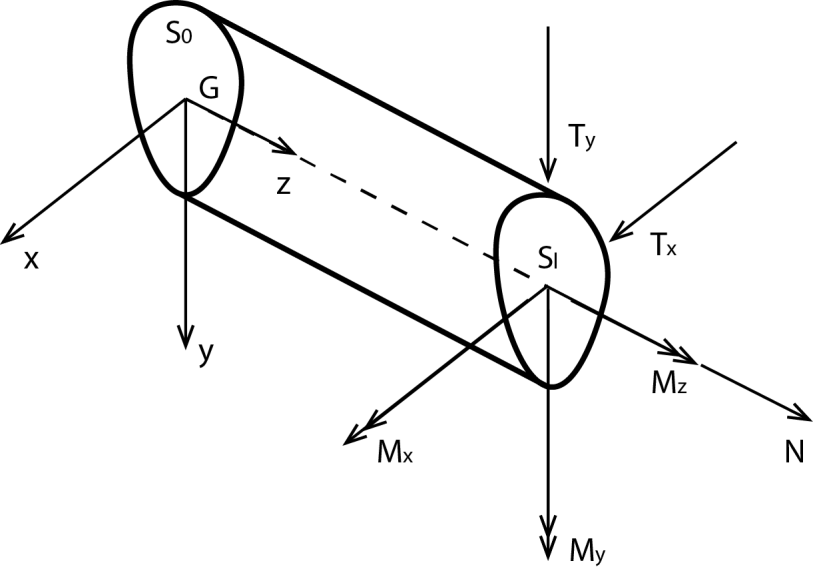
\includegraphics[width=0.3\linewidth]{immagini/screenshot002}
			\label{fig:screenshot002}
		\end{figure}
				
		L'intaglio genera una perturbazione tale nello stato tensionale da trasformare uno stato di tensione monodimensionale, ad uno bi- o tridimensionale, non solo altera una tensione principale amplificandola ma ne perturba addirittura le componenti. \newline 
		
		Senza intaglio si vede bene come al massimo $\sigma_a = \sigma'_a$ costante, mentre con l'intaglio si ha un'amplificazione che arriva a $\sigma_{max}$, il massimo valore che ci si ritrova sul pezzo, proprio in prossimità della pelle della gola, tale valore decrescerà arrivando al cuore del componente, lontano dal taglio tende a ritornare ad un valore nominale, quello che si avrebbe in assenza di intaglio. 
		Al tempo stesso però, insieme ad una tensione assiale, nel caso del cilindro con gola nascono delle componenti radiali e tangenziali non nulle, anche se più basse rispetto a quella assiale. 
		
		Perché la componente radiale parte da $0$ e ritorna a $0$? Deve essere rispettata la condizione al contorno, poiché non esistono componenti di sezione ortogonali alla superficie, se non c'è carico la componente normale dev'essere nulla, in questo caso la componente normale corrisponde a quella radiale, che dovrà essere nulla. \newline
		
		
		Altro esempio può essere fornito dalla lastra forata posta in trazione. 
		
		\begin{figure}[H]
			\centering
			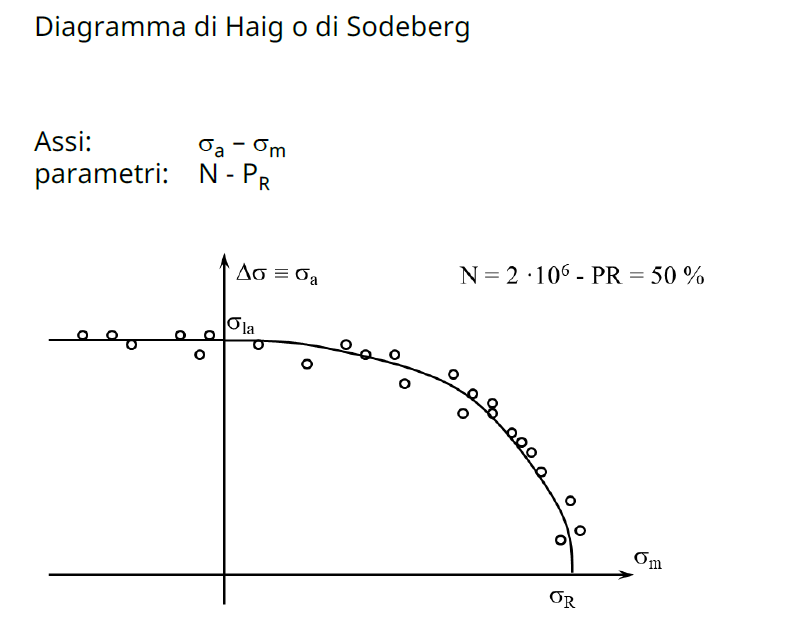
\includegraphics[width=1\linewidth]{immagini/screenshot003}
			\label{fig:screenshot003}
		\end{figure}
				
		Lontano dal foro il carico applicato genera una tensione costante  $\sigma_0$ uniforme, come viene perturbata questa tensione appena ci si avvicina al foro? 
		
		Siano $\sigma_r$ e $\sigma_\theta$ rispettivamente le tensioni radiali e tangenziali. \newline 
		
		La tensione lungo $x$ al variare della quota $y$, se non ci fosse un effetto di concentrazione di tensione sarebbe quella verticale tratteggiata, leggermente superiore a $\sigma_0$ perché essendoci l'intaglio, la sezione resistente è minore: stesso carico su area ridotta = tensione nominale maggiore. 
		
		Rispetto a quella $\sigma_0$ l'andamento delle componenti circonferenziali ha un picco sulla pelle del foro e poi decresce. 
		
		\begin{figure}[H]
			\centering
			\begin{tikzpicture}[>=latex]
			%%%	Help Lines
%			\draw [thin, help lines] (0,0) grid (10,10);
%			\foreach \x in {0,...,10}
%			\draw (\x cm,1pt) -- (\x cm,-1pt) node[anchor=north] {$\x$};
%			\foreach \y in {0,...,10}
%			\draw (1pt,\y cm) -- (-1pt,\y cm) node[anchor=east] {$\y$};
			%%%	Disegno	
			\draw (5,5) arc (0:-90:5 and 3);
			\node[above] at (5,5) {$0$}; 
			\node[left] at (0,2) {$\max$};
			\node [draw, circle] at (5,3.5) {+};
			\draw[->] (6,5) -- (5,5);
			\draw[->] (6,4) -- (4.75,4);
			\draw[->] (6,4) -- (4.75,4);
			\draw[->] (6,3) -- (3.75,3);
			\draw[->] (6,2) -- (0,2);
		\end{tikzpicture}
		\end{figure}
		
		Quelle radiali sono molto piccole, partono da $0$ e arrivano a $0$ per rispettare le condizioni al contorno e hanno una perturbazione vicino al foro, sotto pelle, ad una certa profondità nel materiale in direzione radiale rispetto alla superficie. Questo è un problema che concernerà usura e corrosione. 
		
		\begin{figure}[H]
			\centering
			\begin{tikzpicture}[>=latex]
			%%%	Help Lines
%			\draw [thin, help lines] (0,0) grid (10,10);
%			\foreach \x in {0,...,10}
%			\draw (\x cm,1pt) -- (\x cm,-1pt) node[anchor=north] {$\x$};
%			\foreach \y in {0,...,10}
%			\draw (1pt,\y cm) -- (-1pt,\y cm) node[anchor=east] {$\y$};
			%%%	Disegno	
			%	\draw (5,10) arc (90:270:2);
			\draw (5,10) .. controls (1,8) and
			(4.5,6) .. (5,0);
			\node[above] at (5,10) {$0$}; 
			\node [draw, circle] at (5,8) {+};
			\node[below]  at (5,0)  {$0$}; 
			\draw[->] (6,9) -- (3.65,9);
			\draw[->] (6,7) -- (3.25,7);
			\draw[->] (6,6) -- (3.5,6);
		\end{tikzpicture}
		\end{figure}
		
		Come variano invece le tensioni in direzione $x$? In direzione radiale, a causa delle condizioni al contorno sul foro, partono da $0$ e come ci si allontana dallo stesso diventerà pari a $\sigma_0$, finisce la perturbazione. 
		
		\begin{figure}[H]
			\centering
			\begin{tikzpicture}[>=latex]
			%%%	Help Lines
%			\draw [thin, help lines] (0,0) grid (10,10);
%			\foreach \x in {0,...,10}
%			\draw (\x cm,1pt) -- (\x cm,-1pt) node[anchor=north] {$\x$};
%			\foreach \y in {0,...,10}
%			\draw (1pt,\y cm) -- (-1pt,\y cm) node[anchor=east] {$\y$};
			%%%	Disegno	
			\draw (5,5) arc (180:90:5 and 3);
			\node[below] at (5,5) {$0$}; 
			\node[right] at (10,8) {$\max$};
			\node [draw, circle] at (8,6) {+};
			\draw[->] (6,4) -- (6,6.75);
			\draw[->] (7,4) -- (7,7.25);
			\draw[->] (9,4) -- (9,7.95);
		\end{tikzpicture}
		\end{figure}
\newpage		
		La componente circonferenziale invece lontano dal foro andrà sicuramente a $0$ perché banalmente non si hanno componenti circonferenziali, mentre in prossimità del foro subirà una piccola tensione di compressione che diverrà a trazione e si annullerà per quanto appena detto. 
		
		\begin{figure}[H]
			\centering
			\begin{tikzpicture}[>=latex]
			%%%	Help Lines
%			\draw [thin, help lines] (0,0) grid (10,10);
%			\foreach \x in {0,...,10}
%			\draw (\x cm,1pt) -- (\x cm,-1pt) node[anchor=north] {$\x$};
%			\foreach \y in {0,...,10}
%			\draw (1pt,\y cm) -- (-1pt,\y cm) node[anchor=east] {$\y$};
			%%%	Disegno	
			\draw (0,5) -- (9,5);
			\draw (0,5) .. controls (5,5) and
			(7,10) .. (8,2);
			\node [draw, circle] at (6,6) {+};
			\node [draw, circle] at (8.25,4) {-};
			
			\draw[->] (4,4) -- (4,5.95);
			\draw[->] (5,4) -- (5,6.25);
			\draw[->] (7,4) -- (7,5.7);
			\draw[->] (7.75,3.65) -- (7.75,5);
		\end{tikzpicture}
		\end{figure}
		
		Questo appena trattato è uno dei pochi esempi per cui si può trovare la soluzione analitica, ma serve la teoria dei dischi. È un esempio però in cui l'approccio con $K_t$ dice soltanto quanto vale la tensione, e non gli importa delle perturbazioni che avvengono in tutti gli altri punti. \newline 
		
		\textbf{{\Large Determinazione del fattore di concentrazione degli sforzi }} \newline 
		Come si quantifica il $K_t$? Il $K_t$ su geometrie ben progettate non è mai superiore a 4 , magari una flangia va imbullonata e dei fori passanti ci vorranno sempre, si può anche giocare con gli effetti mutui dati dalla vicinanza di fori, per cui la perturbazione delle tensioni viene calmierata, ma non impedirà alle concentrazioni di tensione di esistere. 
		
		Se il componente non è ben progettato e ci sono difetti o danni il $K_t$ può tendere a valori estremamente elevati, per cui giocoforza sarà soltanto un valore teorico: un $K_t=1000$ non ha tutto questo gran senso fisico, si ha sull'apice di una cricca, su di un impatto, con una concentrazione tale il materiale o si è fotto o si è fortemente plasticizzato. \newline 
		
		L'approccio col fattore di concentrazione è dunque limitativo e il suo calcolo può essere effettuato in maniera analitica in forma chiusa in pochissimi casi, si potrà ricorrere a metodi numerici agli elementi finiti, la cui soluzione dipenderà però dal grado di dettaglio utilizzato nel modello, ma sarà sempre una soluzione approssimata. 
		
		Si potranno eseguire prove sperimentale di fotoelasticità, estensimentria o attraverso l'utilizzo di vernici fragili, quest'ultimo approccio si basa sull’impiego di una speciale vernice che si frattura
		quando la deformazione supera un valore limite.
		
		Vengono esaminate quindi le isostatiche e si risale alle
		tensioni principali, proporzionali al valore limite di rottura. \newline
		
		L'approccio col $K_t$, siccome si basa sul concetto che la massima tensione è quella che porta a rottura, trova interesse d'applicazione soprattutto sui materiali fragili. Sui materiali duttili in condizioni di sollecitazione statiche, il progettista è chiamato ad ignorare il $K_t$. \newline 
		
		Il criterio del $K_t$ è infatti chiamato \textbf{criterio di picco}: si usa il picco di tensione per il confronto con l'ammissibile. 
		\[\sigma_{max} = K_t\sigma_{nom}\leq\sigma_{amm}\]
		
		Molto spesso il modo con cui si arriva a criticità col materiale duttile è più complesso, dipende dalla distribuzione di tensioni tangenziali, dipende dall'energia di deformazione se questa viene usata a dilatare o a distorcere: il coefficiente $K_t$ per materiali duttili è approssimato e approssimativo. 
		
		Si utilizzano allora \textbf{criteri di campo} in cui in prossimità dell'apice di una cricca non si valuta il valore puntuale, ma si valuta una distribuzione di tensione, questo è un criterio che implica una modellistica data dalla teoria della meccanica della frattura. \newline 
		
		Approcci più pratici si basano sul presupposto che il pezzo sia reale e quindi prima o poi snerverà da qualche pare, d'altro canto è un utopia pensare di avere comportamento perfettamente elastico ovunque nel componente in presenza di variazioni di forma anche spinte. Si parte perciò da presupposto che il materiale raggiunga uno snervamento nella prossimità dell'intaglio che porterà a plasticizzazione locale. Tale plasticizzazione locale dovrà essere molto contenuta in termini di volume di materiale interessato, tanto da non impattare il comportamento globale del componente: se la sezione risultante si comporta ancora in maniera elastica, l'andamento sarà allora grossomodo elastico, se invece la plasticizzazione è più estesa il problema cambia. \newline 
		
		Un approccio di criticità potrebbe essere quello della \textbf{plasticizzazione totale} della sezione resistente: è necessario porre l'attenzione che la totalità della sezione o buona parte di essa abbia raggiunto la la plasticizzazione, perché in quel caso se il comportamento del materiale fosse elastico perfettamente plastico tenendo il carico costante questo continuerebbe a fluire, raggiungendo il plateau del comportamento elastoplastico del materiale. \newline 
		
		L'ultimo approccio utilizzabile è quello della \textbf{plasticizzazione vera}, sviluppato questo con metodi numerici, riesce a portare al risultato in termini ragionevolmente brevi, si effettua il calcolo elastoplastico, determinando l’effettivo valore della tensione e deformazione raggiunta, si configura come un approccio di verifica finale definitiva. \newline 
		
		Come detto, il $K_t$ perde di significato quando il materiale è duttile. Ad esempio non ha senso usare un $K_t=4$ quando la tensione nominale è già all'80\% dello snervamento, un materiale elastico perfettamente plastico se raggiunge lo snervamento non offre più alcuna resistenza, quel surplus di carico che quella parte di materiale non è più in grado di sopportare viene indirizzata verso il materiale subito accanto. Se si continua a caricare il materiale, questo offre una tensione superiore allo snervamento? Ovvio che no, il plateau del comportamento del materiale dice che qualunque elemento del materiale al massimo raggiunge lo snervamento , più di così non può dare. L'approccio col $K_t$ per un materiale duttile è perciò puramente teorico. \newline 
		
		Quindi, piuttosto che il $K_t$, per un materiale duttile si preferisce usare un coefficiente d'intaglio $K_{intaglio}$, mettendo a fuoco ora non più il rapporto tra la tensione massima su quella nominale, ma il carico limite sul pezzo qualora non ci fosse intaglio e il carico limite qualora ci fosse intaglio. 
		\[K_{intaglio} = \dfrac{\text{carico limite senza effetti d'intaglio}}{\text{carico limite con effetti d'intaglio}} = \dfrac{\sigma_{amm, senza intaglio}}{\sigma_{amm, con intaglio}}\]
		Parlando di carico e non più di tensione si sta spostando oltre l'orizzonte, non interessa più sapere un rapporto tra tensione nominale e reale, ora interessa sapere solo la variazione di comportamento, non è più un fattore di concentrazioni della singola tensione ma un fattore che tiene conto di come si comporta il materiale. \newline 
		
		Andare a plasticizzazione con un materiale è un discorso che comincia dalla plasticizzazionedella sesione resistente che sono quando è plasticizzata manderà a cedimento il pezzo, al materiale fragile invece basta che in un punto si raggiunga la rottura per vedere. 
		
		Tant'è che per materiali fragili  
		\[k_{intaglio} = K_t\]
		Mentre per i materiale duttili 
		\[k_{intaglio} \approx 1\]
		\begin{proof}
			Sia un materiale duttile in condizioni standard a cui è applicata una sollecitazione statica applicata orizzontalmente. 
			
			\begin{figure}[H]
				\centering
				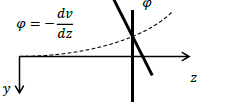
\includegraphics[width=0.5\linewidth]{immagini/screenshot004}
				\label{fig:screenshot004}
			\end{figure}
			
			
			Senza l'effetto dell'intaglio ci si aspetta una tensione nominale costante $\sigma_{no}$ come quella tratteggiata, essendoci l'intaglio l'andamento sarà variabile con un massimo sulla pelle del foro. Si immagini ora di incrementare il carico poco alla volta fino a far raggiungere al massimo, al picco, lo snervamento per comportamento duttile, incrementando il carico in quel punto oltre la tensione di snervamento raggiunta passerà al materiale subito accanto che conserva ancora il comportamento elastico, punto $A$, continuando ad aumentare il carico si arriverà in  $B$, in $C$ fino a quando tutta la sezione raggiungerà lo snervamento, quello sarà il momento critico per il quale incrementando ancora la forza  non c'è più alcuna sezione resistente e il materiale se è idealmente elastico perfettamente plastico fluisce all'infinito. \newline 
			
			Quanto vale in carico limite qualora non ci fossero gli effetti d'intaglio?  Considerando un'area resistente data da:
			\[A_R = (h-d)s\]
			Una tensione di snervamento pari a $\sigma_s$, il carico limite vale, secondo la trave trazionata di De Saint Venant: 
			\[P_L = \sigma_sA_R\]
			
			Qualora invece ci fossero effetti d'intaglio il carico cresce e plasticizza sul foro, ma non è sufficiente a rompere il pezzo, cresce ancora interessando via via sezioni minori, proprio come accaduto in precedenza  finché non arriva a tutta la sezione, in quel momento il carico altro non è che \[P'_L = \int_A\sigma = \sigma_sA_r\] Il coefficiente d'intaglio è:
			\[K_{intaglio} = \dfrac{\text{carico limite senza effetti d'intaglio}}{\text{carico limite con effetti d'intaglio}} = {P_L\over P'_L} = 1\]
			
			E per materiali fragili? Si ripete l'esatto ragionamento. 
			
			\begin{figure}[H]
				\centering
				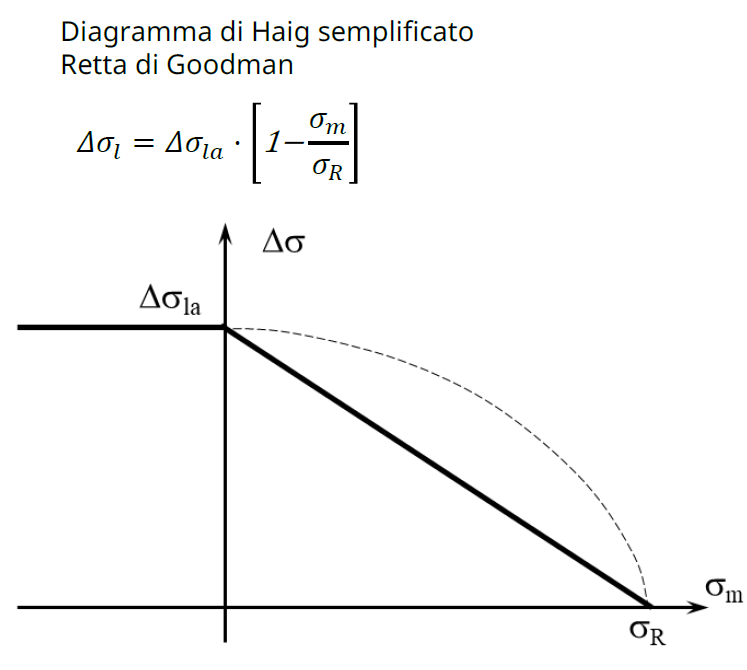
\includegraphics[width=0.5\linewidth]{immagini/screenshot005}
				\label{fig:screenshot005}
			\end{figure}
						
			Il materiale fragile arriverà a rottura in condizioni senza intaglio quando il carico uniforme sulla sezione cresce uniformemente in ogni punto fino a raggiungere il carico di rottura $\sigma_R$. In assenza di effetti di intaglio l'area resistente $A_R$ avrà distribuzione di tensione uniforme che cresce fino a raggiungere il carico di rottura, il carico limite sarà allora sempre pari a:
			\[P_L = \sigma_RA_R\]
			
			In presenza dell'intaglio cosa cambia? C'è un andamento con un picco, il carico crescendo raggiunge un picco dato dal carico di rottura, ora questo è sufficiente a mandare il materiale in condizione critica? Ovvio che si. Per la teoria della meccanica della frattura, se il materiale fragile si rompe in un punto si propaga quasi istantaneamente una cricca in direzione ortogonale al carico che in pochi istanti fa cedere il componente. 
			
			La criticità si ottiene così quando il carico nominale moltiplicato per il coefficiente $K_t$ teorico raggiunge la tensione di rottura: 
			\[\sigma_R = K_t\sigma_{no} = K_t{P_L\over A_R}\]
			Allora:
			\[P'_L = {A_R\sigma_R\over K_t}\]
			Il coefficiente d'intaglio è:
			\[K_{intaglio} = \dfrac{\text{carico limite senza effetti d'intaglio}}{\text{carico limite con effetti d'intaglio}} = {P_L\over P'_L} = K_t\]
			 	 
		\end{proof}
		
		In realtà gli effetti differiscono in base alla tipologia di sollecitazione. 
		
		
		La formulazione di Niemann porta a parametrizzare il carico critico per una determinata geometria in funzione del tipo di sollecitazione, in base a coefficienti noti estrapola i carichi critici. 
		
		\[\begin{aligned}
			P_L & = \nu {A_R\sigma_L\over K_t} \hspace{0.5cm} 1<\nu<K_t \\
			\nu & = 1 + 0.75c \cdot (K_t -1)\left(300\over \sigma\right)^{0.25}
		\end{aligned} \]
		In cui:
		\[\begin{cases}
			c = 1 ~ \text{per trazione e compressione} \\
			c = 1.7 ~ \text{per flessione su provino cilindrico} \\
			c = 1.5 ~ \text{per flessione su provino piano } \\
			c = 1.3 ~ \text{per torsione usando in questo caso $\sigma/0.577$ o $\sigma_{0.2}/0.577$}			
		\end{cases}\]
		
		
		\includepdf[pages=11-13]{08_fcm_2022}
		
		
		
		 
		
		
		
		
	
 		
 		
 		
 		
 		
 		
 		
 		
	 	
	 	
	 	
	 	
	 	
	 	
	 	
		 
		 
		 
	\newpage
	{\Large \textbf{NOTE}}
%	\vfill
%\begin{tcolorbox}[height=4.5cm]
%	This box has a height of 4.5cm.
%\end{tcolorbox}

%DA DECOMMENTARE PER AVERE LA VERSIONE STAMPABILE A DUE PAGINE 	
%	\newpage
%		\null
%		\vfill
%\begin{tcolorbox}[height=4.5cm]
%	This box has a height of 4.5cm.
%\end{tcolorbox}
		\end{adjustwidth}

\end{document}